%complete
\section{Point Cloud Stitching}
\label{design:registration}
\label{design:sitching} %legacy, do not remove
\label{design:stitching}
The specification states that only a single scanner is to be used. This necessitates the utilisation of multiple scans and the stitching thereof into one unified data structure. This data structure can then be manipulated to produce volume estimation, as described in Section \ref{design:volume estimation}. The process of stitching these point clouds together to create one unified dataset is known as \emph{registration}\cite{Makadia2006} which has been described in Section \ref{research:registration}. The development of ideas leading to the final algorithm will be described in this section.  \\

\subsection{Input Data}
Depth maps of people (shells) are to be passed to the registration algorithm from a \emph{person isolation} subsystem. 

\subsection{Design Pattern}
\label{design:design pattern}
The various point cloud stitching algorithms all extend a class called ``Stitcher``. This makes it easy for new stitching algorithms to be deployed within the PARSE environment as only a single line of code needs to be modified in order to use a different stitching algorithm.\\

\subsection{Initial Experimentation}
Initially the point clouds were stitched by rotating successive scans 90\degree \ , increasing by a further 90\degree \ for each previous scan that has been taken, in an anticlockwise direction. The scan was then translated by a constant vector to produce a reasonable point cloud. This was able to produce reasonable results in individual cases but people come in a variety of ``depths`` and such an algorithm would only be useful in a world where everyone had constant "depths". \\

\subsection{Development of a more sophisticated approach: Bounding Boxes} 
\label{design:bounding boxes}
\label{design:bounding box}
While the Kinect is designed to produce depth information, it is only capable of scanning the visible surfaces of objects in front of the point in the 3D world in which it is situated. This has led to the coining of the term \emph{2.5D} to explain the limited information that the Kinect, and all single depth sensors, are able to gain about the world around them \cite{lu2006}. In theory this very limitation can be exploited to produce a reasonable, but by no means perfect, point cloud registration most cases. Within the context of this project this has come to be known as the \emph{Bounding Box} method of point cloud registration. \\ 

\subsubsection{Scanning Phase}
As with the initial experimentation, the bounding box method requires four scans; $S_1, S_2, S_3, S_4$. After each scan is obtained the patient is rotated by 90\degree \ in an anti clockwise direction. Each scan contains length and width information which is used in the processing phase. These scans are then packaged into a list data structure and sent to the bounding box method for processing. \\

\subsubsection{Processing Phase}
The processing phase consists of a number of simple rotations and translations. The subject was only rotated about the vector $(0, 1, 0)$ which significantly reduced the complexity of the operations. Table \ref{tab:bb processing} shows the rotations and translations that were performed for each scan. \\

%table 
\begin{table}
    \begin{tabular}{| p{0.8cm}| p{1.4cm} | p{4.9cm} | p{3.9cm} |}
    \hline
        Scan & Rotation & Rotation Axis & Translation  \\
        \hline
        $S_1$ & 0 \degree & $(0, 0, 0)$ & (0,0,0)  \\
        $S_2$ & 90 \degree & $(S_2(x_{min}), S_2(y_{min}), S_2(z_{min}))$ & $(0, 0, width)$  \\
        $S_3$ & 180 \degree & $(S_3(x_{min}), S_3(y_{min}), S_3(z_{min}))$ & $(S_3(width), 0, S_2(width))$  \\
        $S_4$ & 270 \degree & $(S_4(x_{min}), S_4(y_{min}), S_4(z_{min}))$ & $(S_3(width), 0, 0)$  \\
        \hline
    \end{tabular}   
    \caption{The processing that takes place on each data item for the Bounding Box method}
    \label{tab:bb processing}
\end{table} \\

\subsubsection{Challenges}
Despite the apparent successful stitching in many cases, the \emph{Bounding Box} method produced erratic results occasionally. Due to anatomical differences, male subjects tended tended to be stitched more accurately than female ones. This was also the case with obese subjects. This problem has been internally known as the \emph{Breast Problem} (Section \ref{testing:the breast problem}). \\

To address this; a more sophisticated registration method, the Iterative Cloud Positioning (ICP) algorithm (Discussed in Section \ref{res:icp}) was investigated. One of the big problems with the ICP algorithm, and other registration algorithms, is that they require some form of initial alignment which is then improved over time. This initial problem had already been potentially solved using the Bounding Box method and so it has been utilised part of a processing pipeline. \\

\subsection{Manual Alignment}
As discussed in the previous section, it is necessary that some form of initial alignment is made before most algorithms would be useful. To address the breast problem (Section \ref{testing:the breast problem}) it could be possible to offer some kind of manual alignment of the body panels. This, however, would potentially introduce unpredictable human error and would require real-time visualisation and modification of the point cloud data structures. Performing just four rotations and one rendering, as in the Bounding Box method \ref{design:bounding box}, takes several seconds to complete and therefore a new trade-off of image resolution vs display and processing hardware would be introduced. The manual alignment idea was ultimately abandoned due to the overriding objective of keeping the final product cheap in terms of hardware requirements, accurate and easy for the operator to use. \\

\begin{figure}[h!!]
    \label{fig:registration pipeline}
    \begin{center}
        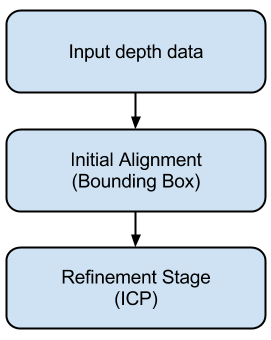
\includegraphics[scale=0.6]{zscreenshots/reg-pipeline.png}
        \caption{A pipelined approach towards registration}
    \end{center}
\end{figure}

\subsection{Final design: Iterative Closest Point (ICP) algorithm}
So far it has been explained how a simple method that is the bounding box method is able to produce reasonably good results. In Section \ref{res:icp} we learnt that the gold standard for registration is the Iterative Closest Point method which requires some initial alignment. This alignment could be provided by the bounding box method. \\ 

Using the information that from experimentation and the research in Section \ref{res:icp} a pipelined approach to registration was developed using the three steps, explained in Figure \ref{fig:registration pipeline}.

